\section{Задание 2. Формула Тейлора.}
\textbf{Условие.}

Дана функция $\displaystyle y = f(x) = cos^2 \frac{x}{2}, \quad x_0 = 0, \quad dx = 5^\circ, \quad \delta = 0.01, \quad \varepsilon = 10^{-5}$\\
\begin{enumerate}
    \item Найдите формулу её производной $n$–го порядка.
    \item Представьте функцию формулой Тейлора $n$-го порядка в окрестности точки $x_0$. Обозначьте остаточный член $R_n(x)$, если многочлен Тейлора имеет степень $n$.
    \item Используя полученное представление и данные в таблице:
    \begin{enumerate}
        \item Запишите уравнение касательной к функции в точке $x_0$. Сделайте вывод о характере монотонности функции в окрестности точки $x_0$.
        \item Запишите $R_n(x)$ в форме Пеано. Найдите радиус окрестности $x_0$, в каждой
        точке которой значение дифференциала $dy$ отличается от приращения функции
        $\Delta y$ не более, чем на $\pm \delta$.
        \item Запишите $R_n(x)$ в форме Лагранжа. Определите знак(и) остатка $R_1(x)$ на
        интервале $(x_0 - dx, x_0 + dx)$. Сделайте вывод о взаимном расположении
        касательной и графика функции. Что можно сказать о выпуклости и перегибах
        функции на этом интервале?
        \item Найдите, какой степени $n$ должен быть многочлен Тейлора, чтобы представлять
        функцию в точке $x = x_0 + dx$ с точностью $\varepsilon$. Найдите значение функции в
        точке $x$ с заданной точностью.
    \end{enumerate}
    \item Постройте графики функции, многочлена Тейлора и остатка. Сверьте с графиками
    результаты аналитического исследования. Образец построения здесь.
\end{enumerate}
\vspace{10mm}
\textbf{Решение.}

\begin{enumerate}
    \item Формула производной n-ого порядка

    $\displaystyle y = cos^2 \frac{x}{2} = \frac{1 + \cos x}{2} = \frac{1}{2} + \frac{1}{2} \cos x$

    $y' = \displaystyle -\frac{1}{2} \sin x\quad$
    $y'' = \displaystyle -\frac{1}{2} \cos x\quad$
    $y''' = \displaystyle \frac{1}{2} \sin x\quad$
    $y'''' = \displaystyle \frac{1}{2} \cos x$

    Видим зацикливание:
    $y^{4n} = \displaystyle -\frac{1}{2} \sin x\quad$
    $y^{4n + 1} = \displaystyle -\frac{1}{2} \cos x\quad$
    $y^{4n+2} = \displaystyle \frac{1}{2} \sin x\quad$
    $y^{4n+3} = \displaystyle \frac{1}{2} \cos x$

    \item Формула Тейлора

    $\displaystyle f(x) = f(0) + f'(0)x + \frac{f''(0)x^2}{2!} + \frac{f'''(0)x^3}{3!} + \frac{f''''(0)x^4}{4!} + \dots = 1 - \frac{x^2}{2 * 2!} + \frac{x^4}{2 * 4!} + \dots$

    $\displaystyle f(x) = 1 - \sum_{k=0}^{\lfloor \frac{n - 2}{4} \rfloor}\frac{x^{4k + 2}}{2 * (4k+2)!} + \sum_{k=0}^{\lfloor \frac{n - 4}{4} \rfloor}\frac{x^{4k}}{2 * (4k)!} + R_n(x)$

    \item Всякое с $R_n(x)$

    \begin{enumerate}
        \item Уравнение касательной

        $f'(0) = - \frac{1}{2}\sin(0) = 0$.
        Значит либо функция в окрестности $x_0$ константа, либо она меняет характер монотонности в этой точке. $cos^2 \frac{x}{2}$ не константная функция, значит в окрестости точки 0 она меняет харатер монотонности\\

        \item Пеано

        $\displaystyle  R_n(x) = o((x-x_o)^n) = x^n$

        $\displaystyle  \triangle y = f(\pm \triangle x) - f(0) = \frac{1}{2} \cos \triangle x - \frac{1}{2}$

        $\displaystyle  dy = -\frac{1}{2}\sin(0) dx = 0$

        $\displaystyle  \triangle y - dy = \triangle y < - \delta$

        $\displaystyle \frac{1}{2} \cos \triangle x - \frac{1}{2} < -0.01$

        $\displaystyle \cos \triangle x - 1 < -0.02$

        $\displaystyle \cos \triangle x < 0.98$

        $\displaystyle \triangle x < \arccos (0.98)$

        Это оценка с одной стороны: где $x > 0$.
        Аналогично можно сделать слева от нуля, а можно заметить что cos - четная функция и относительно нуля ее график семтричен. Значит радиус окрестности равен 2 * $\arccos(0.98)$

        \item Лагранж

        $\displaystyle R_1 = -\frac{\frac{1}{2}\cos (c)}{2}x^2$

        $\displaystyle x \in (x_0 -dx; x_0 + dx)$

        $\displaystyle x \in \left(-\frac{\pi}{36}; \frac{\pi}{36}\right)$, $c \in (0; x) \subset \left(-\frac{\pi}{36}; \frac{\pi}{36}\right)$ значит $\cos(c) >= 0$ значит $R_1(x) <= 0$ значит $y(x)$ выпукла вверх и лежит под касательной

        \item нужная степень многочлена Тейлора

        $\displaystyle y(x_0 + dx) = \frac{1 + \cos\left(\frac{\pi}{36}\right)}{2}$

        $\displaystyle n = 6: T(x)_6 - y(x_o + dx) = 1 - \frac{{\frac{\pi}{36}}^2}{2 * 2!} + \frac{{\frac{\pi}{36}}^4}{2 * 4!} - \frac{{\frac{\pi}{36}}^6}{2 * 6!} - \frac{1 + \cos \left(\frac{\pi}{36}\right)}{2} < \delta$

        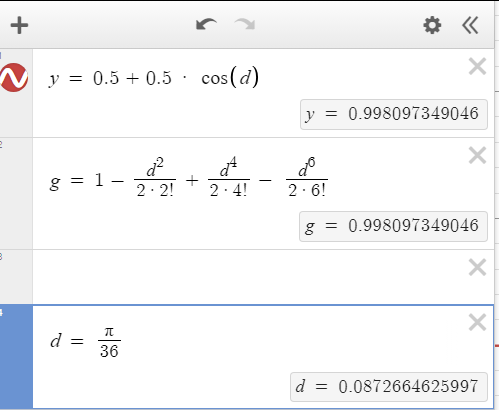
\includegraphics[width=0.55\linewidth]{images/2_check.png}

        Таким образом степени 6 хватает чтобы с заданой точностью приблизиться к значению $\cos(dx + x_0)$ рядами Тейлора

    \end{enumerate}

    \item График

    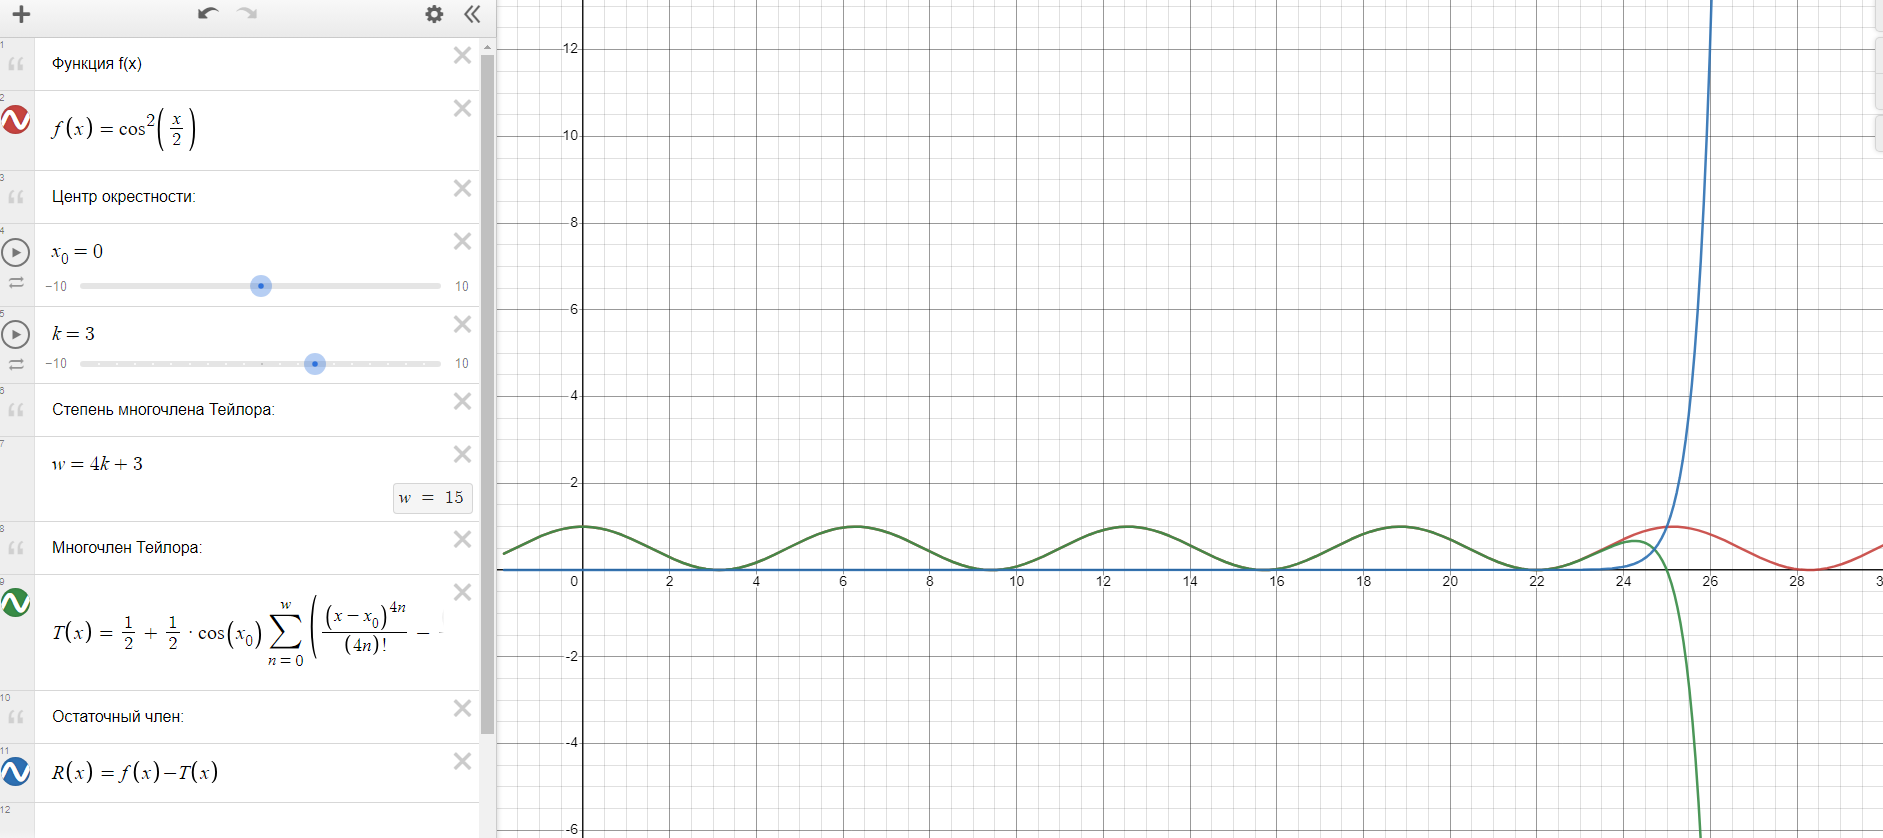
\includegraphics[width=1.0\linewidth]{images/graph.png}

\end{enumerate}

\clearpage
